\chapter{数据准备}
\label{chapter-Data}

\space 本章中,介绍了本文研究内容前期的准备过程,主要分为两部分:基于树状区块链的出租车调度系统的复现、真实地图数据的处理导入。

\section{基于树状区块链的出租车调度系统的复现}

为了利用车联网的地理分区特性,提高区块链存储访问效率,周畅设计了一种按照Geohash编码方式划分的,具备区域物理位置状态特性的树状多链结构\cite{s22228885}。

成佳壮基于该地理位置区块链,设计与实现了出租车调度系统。该系统使用由Geohash编码的地理信息,结合了A*路径规划算法,基于地理位置实现了区域车乘匹配的功能。

万琦玲在该出租车调度系统的基础上,完善了用户接口设计和用户信誉值评估模块设计,完成了车辆行驶状态、信誉评估的可视化效果,并实现了跨设备访问该系统的功能。

基于树状区块链的出租车调度系统的复现工作由实验室的成员一同合作完成,其中实验室其余成员基于树状区块链对成佳壮设计的出租车调度系统完成了复现;本文将以上三人的工作结合,基于树状区块链对万琦玲优化的出租车调度系统进行了复现,重现了基于树状区块链、由Geohash编码地理信息、采用传统A*路径规划算法、完善用户接口设计和信誉值评估模块设计的出租车调度系统的运行效果。

本文的复现工作依赖的设备配置环境为:

1.虚拟机软件:7.0.6版本的VirtualBox。

2.虚拟机的Linux操作系统:22.04版本的Ubuntu。

3.虚拟机基础配置:(1)内存大小设置为5220MB;(2)4核处理器;(3)磁盘空间设置为30.00G。

\subsection{树状区块链}

\space 传统区块链技术中,每个区块仅保存上一个区块的哈希,形成一条单链结构,不具备移动性,无法绑定地理位置信息,因此不能利用车联网的地理分区特性。单链也要求所有节点必须在同一区块链中,导致节点数量、数据量过大,影响区块链存储访问效率,也不符合车联网中车辆节点的移动性。

\space 周畅提出的树状区块链技术基于位置\cite{s22228885},该区块链按照Geohash编码方式划分,具备区域物理位置状态特性。

树状区块链主要包括以下工作:按照Geohash编码的地理区域划分并更改区块数据结构、层次化分类区块与节点、层次化组织区块、区域信息汇总。

% 开始放置单图片
\begin{figure}[ht]
    \centering
    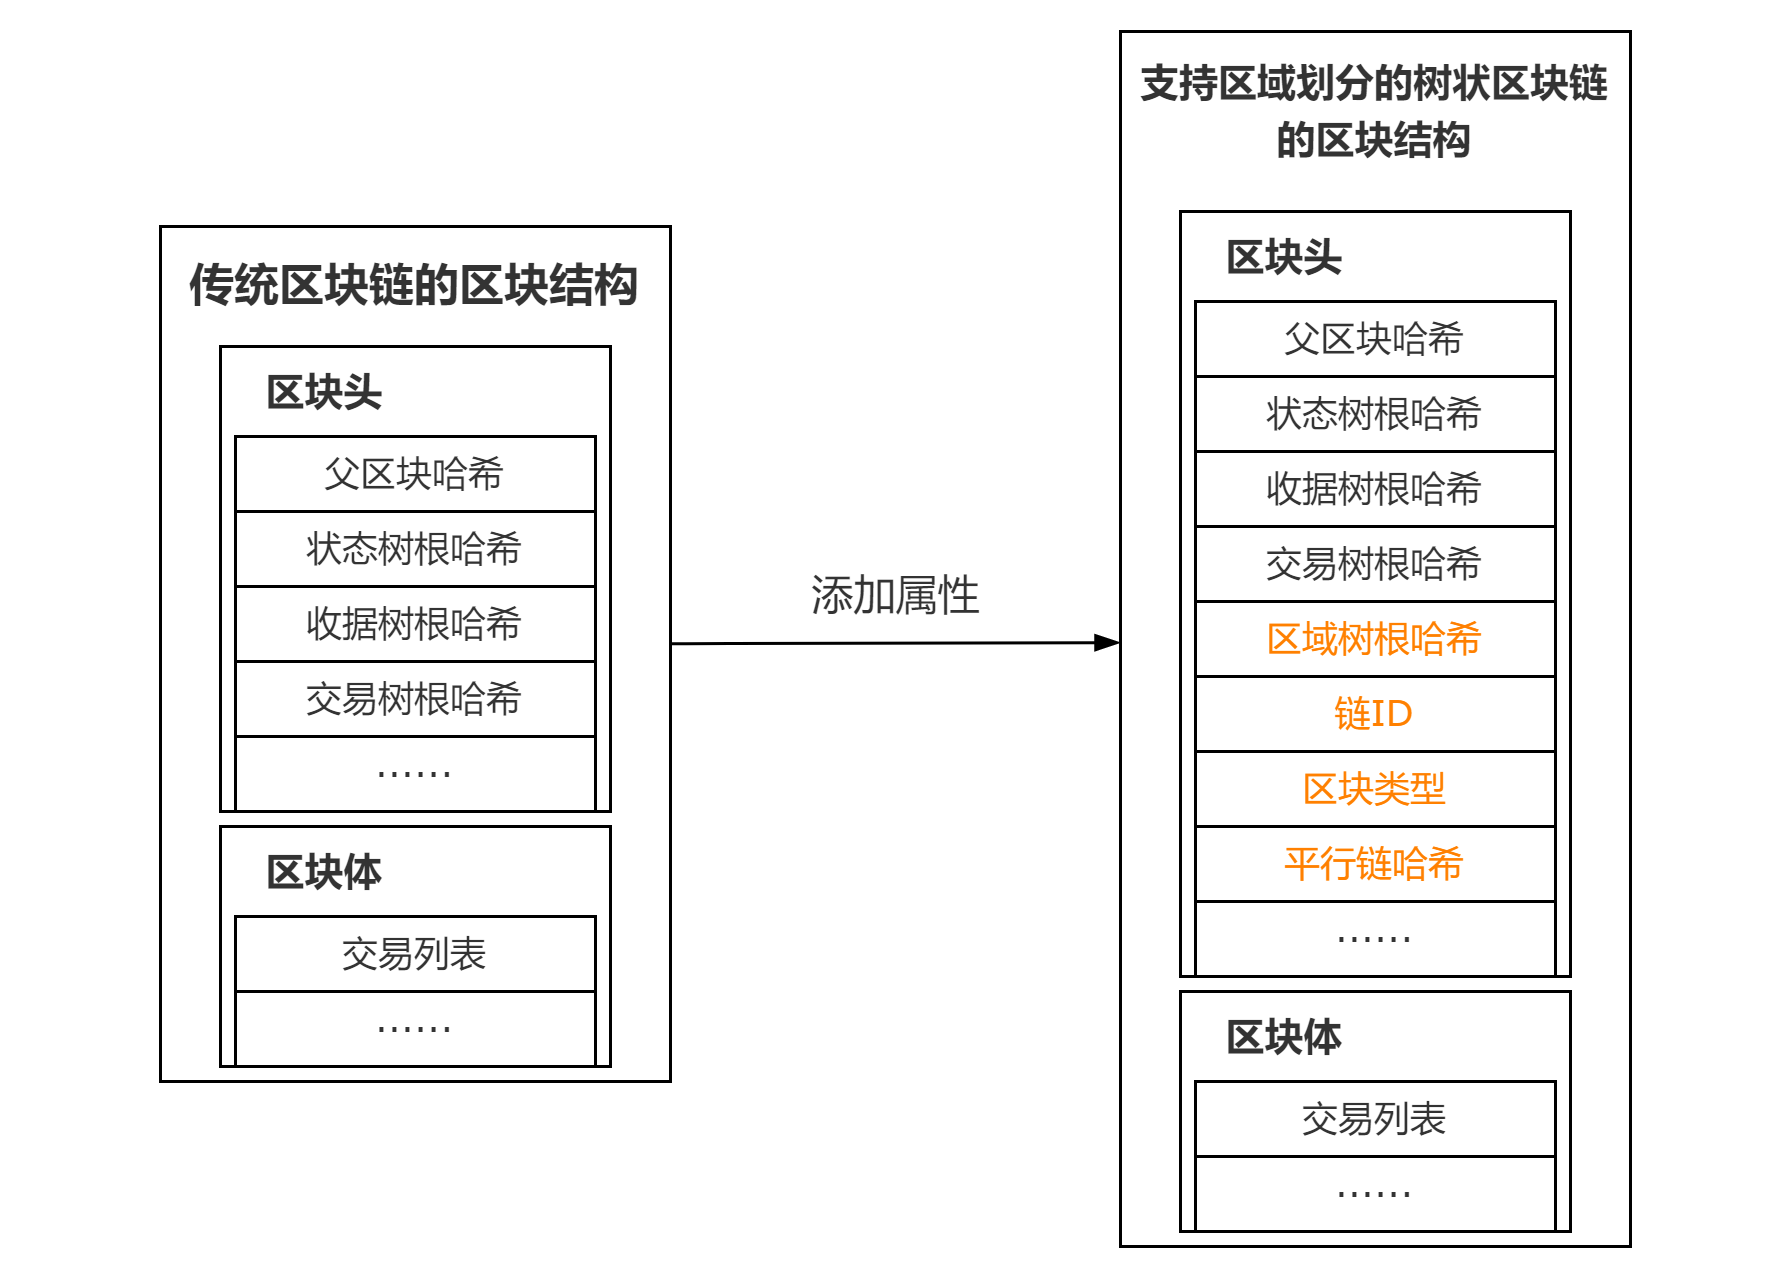
\includegraphics[width=0.8\textwidth]{undergraduate-thesis/images/TreeBlockchainNewProperty.png}
    \caption{支持区域划分的树状区块链结构示意图}
    \label{TreeBlockChain}
\end{figure}
% 结束放置单图片

\begin{enumerate}
    \item 按照Geohash编码的地理区域划分并更改区块数据结构。
    
    如图\ref{TreeBlockChain},相比于传统区块链,树状区块链在区块头中添加了同层块、块类型、链ID、区域根这四个属性。
    \begin{enumerate}
        \item 区域树根哈希:区域状态树(Region State Trie,RST)用于支持查询区域地理位置的相关数据。区域状态树用于记录地理区域内的全局变化,从而便于查询地理信息、验证数据可信。
        \item 链ID(chainID):用于区分来自不同区块链的区块。在多链的结构下,链ID一方面能方便按照不同子链同步区块内容,另一方面也能便利父链对子链的快速查询。
        \item 区块类型(blockType):支持区域划分的树状区块链结构有以下三类区块:创世块、分支区块、普通区块。该属性即对当前区块的类型进行区分。
        \item 平行链哈希(parallel Hash):分支区块用父链指针指向上层区块,用平行链指针指向跟自己拥有相同父区块、且Geohash编码位数相同的已产生的同层级分支区块。这样做便于使分支区块能维护其在树状区块链中的结构关系。
    \end{enumerate}
    \item 层次化分类区块与节点:
    \begin{enumerate}
        \item 区块分类:
        \begin{enumerate}
            \item 创世块:树状区块链结构里的第一个区块。全链的创世块保持一致。
            \item 分支区块:分支区域的第一个区块。在支持区域划分的树状区块链中,每增加一个层级,就增加32个分支区块。
            \item 普通区块:分支区域里的分支区块的子区块,记录对应地理区域内部发生的交易。
        \end{enumerate}
        \item 节点分类:
        \begin{enumerate}
            \item 全节点:维护全区块链完整的区块数据和全局状态树。部分服务器是全节点。
            \item 区域节点:维护其所在区域指定层次及以下的所有分支区块和普通区块。路侧节点和部分服务器是区域节点。
            \item 叶节点:是可以构建分支区块的最底层节点,维护其所在区域最下层的分支区块和普通区块。车辆节点是叶节点。
        \end{enumerate}
    \end{enumerate}
    \item 层次化组织区块:
    
    支持区域划分的树状区块链依据Geohash编码来完成层次化结构的组织。Geohash编码通过二分法将指定区域分为网格,每个网格的编码表示唯一。编码长度越长,则网格越小,对应的地区越精细,层次越低。根据Geohash编码的特性,该树状区块链的层次关系即对应地理区域的包含关系。因此,在该树状区块链中,上层分支区块对应的地理区域中,包含所有以该区块为父块的下层区块对应的地理区域。
    \item 区域信息汇总:

    在支持区域划分的树状区块链中,普通区块打包已发生的交易,分支区块提供子区块链的头区块和索引功能。当子链区块需要同步信息时,分支区块按照子链的地理区域独立进行区块汇总,将每个区域子链的待同步区块添加到分支区块链的对应分支上,并在分支节点处缓存汇总区域状态,以提高查询效率。
    
    支持区域划分的树状区块链融合地理位置,设计与地理位置相关的数据结构,通过Geohash的层级划分方式建立树状的多层级结构。将区块链以Geohash编码的方式,按照地理区域划分成多链,符合车辆节点在行驶过程中只对本区域地图数据感兴趣的特征,减少了每条链中的数据量和节点数量,提高了区块链的存储访问效率。
\end{enumerate}

\space 树状区块链融合地理位置,设计与地理位置相关的数据结构,通过Geohash的层级划分方式建立树状的多层级结构。将区块链以Geohash编码的方式,按照地理区域划分成多链,符合车辆节点在行驶过程中只对本区域地图数据感兴趣的特征,减少了每条链中的数据量和节点数量,提高了区块链的存储访问效率。

\subsection{复现树状区块链并部署合约}

树状区块链基于以太坊开发,其在以太坊底层区块链的基础上修改了数据结构,用go语言编译为新的geth客户端。本节将对支持区域划分的树状区块链进行复现,并在其上完成合约部署。

具体的复现手册地址见附录D。

复现部署树状区块链的过程主要经历以下环节:利用genesis.json文件初始化并启动区块链,新建账户并给账户添加余额,再次初始化区块链,确保账户中余额添加成功。在该过程中,主要需关注如下问题:

\begin{comment}
\begin{figure}[ht]
    \centering
    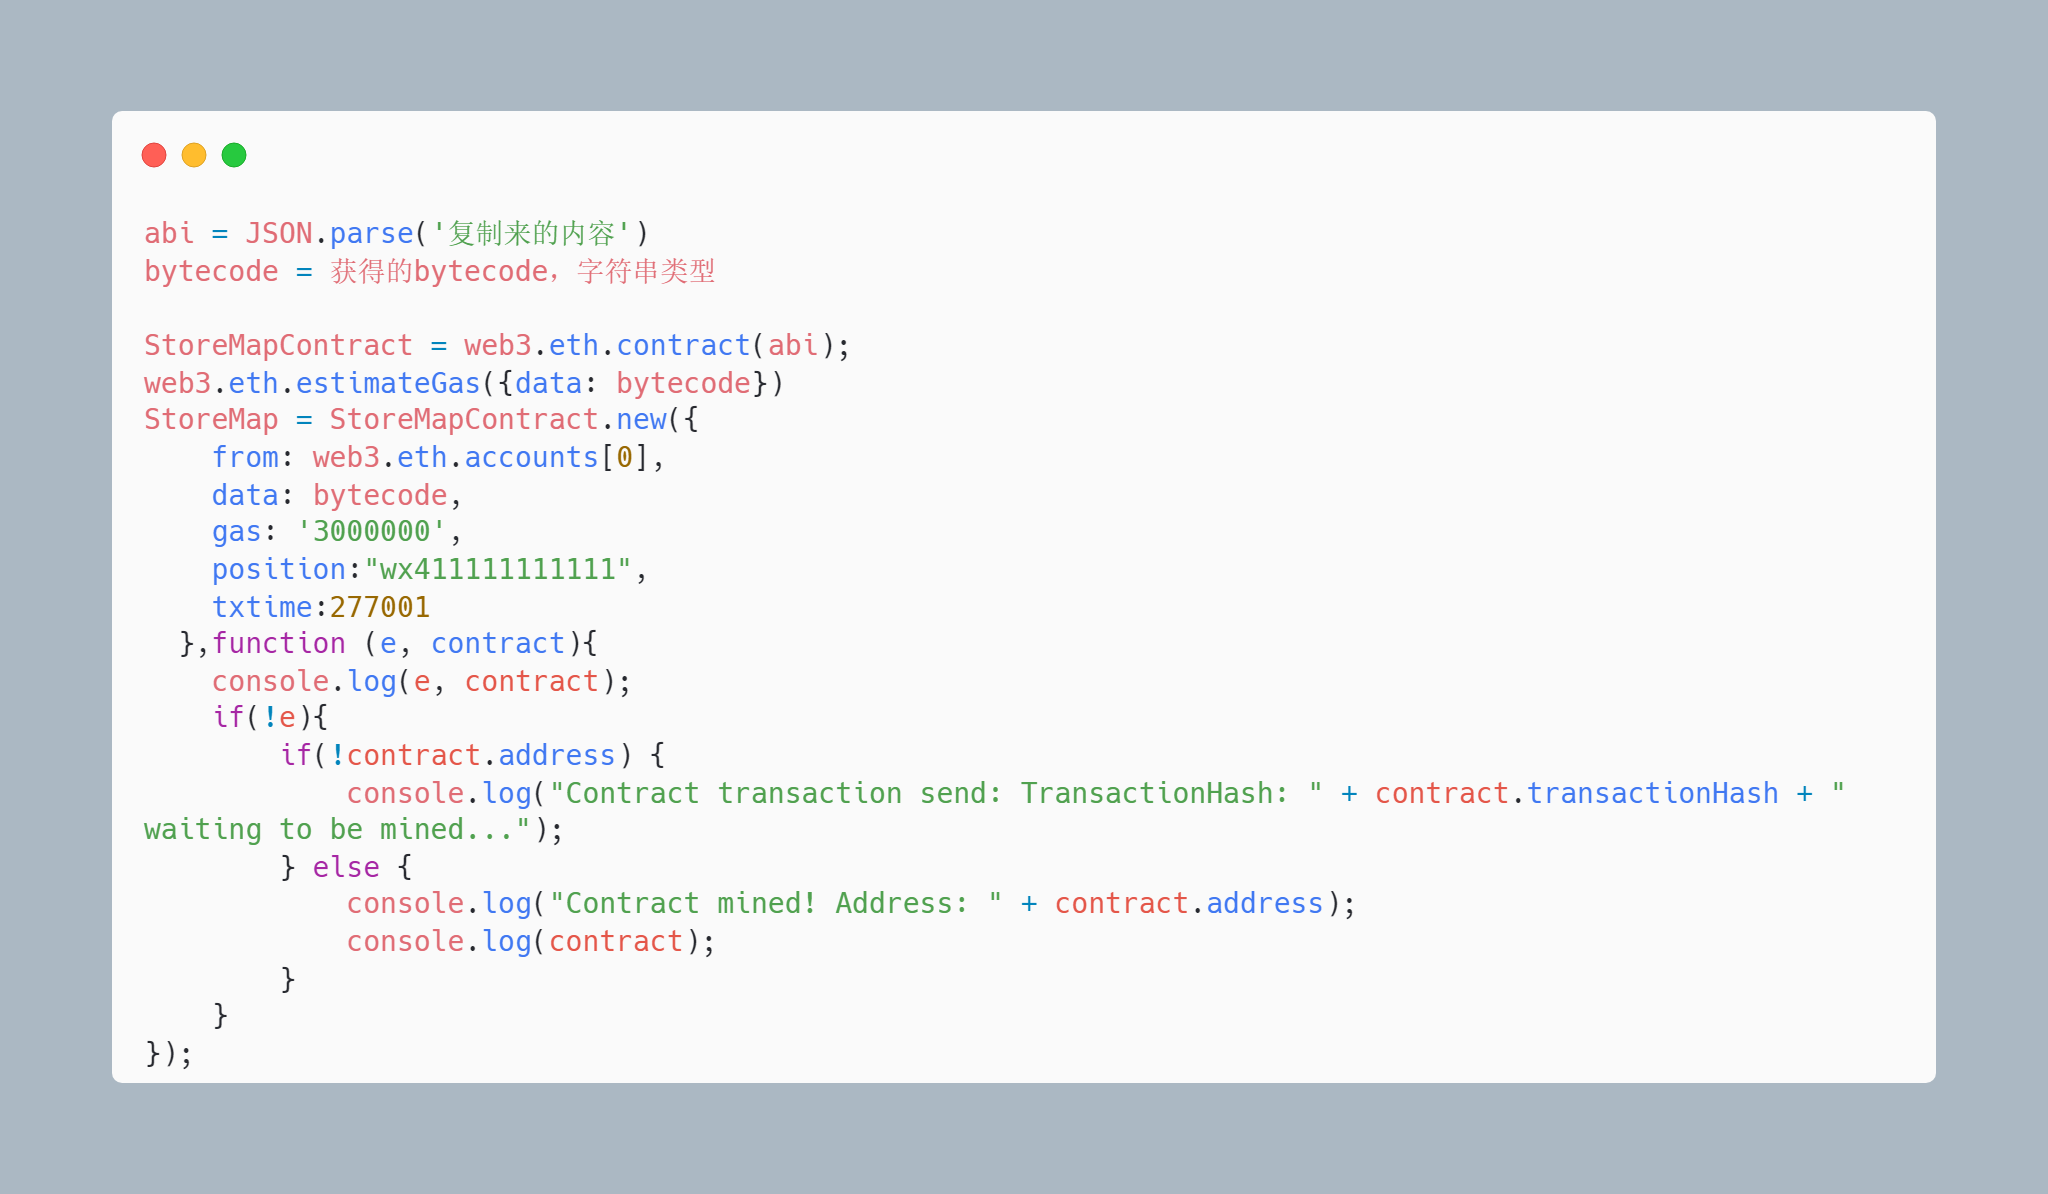
\includegraphics[width=0.7\textwidth]{undergraduate-thesis/images/ContractUpload.png}
    \caption{以StoreMap.sol合约为例的部署代码}
    \label{ContractUpLoad}
\end{figure}
\end{comment}

\begin{enumerate}
    \item 每次重新打开区块链,都需要再解锁一次账户,否则miner.start()无法挖到合约地址。
\begin{lstlisting}[language=java, caption={解锁账户}, label={lst:unlockAccounts}]
    for (i = 0; i < eth.accounts.length; i++) { personal.unlockAccount(eth.accounts[i],"123456",0) }\end{lstlisting}
    \item 在部署合约时,需要格外关注代码2.2中所示的position字段,其需以初始化、启动区块链时,操作语句中的networkid为前缀,否则无法部署到对应树状区块链中。
\begin{lstlisting}[language=java, caption={StoreMap.sol的合约部署代码节选}, label={lst:uploadContract}]
StoreMap = StoreMapContract.new({
    from: web3.eth.accounts[0], 
    data: bytecode, 
    gas: '3000000',
    position:"wx411111111111",
    txtime:277001
},function (e, contract){ }\end{lstlisting}
    
\end{enumerate}

\subsection{复现出租车调度系统}
复现出租车调度系统的过程主要经历以下环节:上传地图、修改脚本里的合约地址和账户名称信息、打开网页接口、启动测试脚本。

具体的复现手册地址见附录D。

在复现过程中,主要需要关注的问题在打开区块链和网页接口部分:

\begin{enumerate}
    \item 首先,要确保区块链的外部访问接口和网络的外部访问接口都已被打开,使用以下语句初始化、启动区块链:
\begin{lstlisting}[language=bash, caption={初始化、启动区块链}, label={lst:initBlockChain}]
    // 初始化区块链
    geth1 --identity "MyEth" --rpc --rpcaddr 0.0.0.0  --rpcport "8545" --rpccorsdomain "*" --datadir gethdata --port "30303" --nodiscover --rpcapi "eth,net,personal,web3" --networkid 91036 init genesis.json
    // 启动区块链
    geth1 --datadir ./gethdata --networkid 91036 --port 30303 --rpc --rpcaddr 0.0.0.0 --rpcport 8545 --rpcapi 'personal,net,eth,web3,admin' --rpccorsdomain='*' --ws --wsaddr 0.0.0.0 --wsport 8546 --wsorigins='*' --wsapi 'personal,net,eth,web3,admin' --nodiscover --allow-insecure-unlock --dev.period 1 --syncmode='full' console\end{lstlisting}
    相比于本地区块链来说,在初始化和启动可被多设备访问的区块链时,需要把代码中的 rpcaddr 127.0.0.1 和 wsaddr=`localhost'修改为 rpcaddr 0.0.0.0 和 wsaddr 0.0.0.0。这样做的目的是为了便于跨设备访问出租车调度系统,否则区块链只被部署在本地,无法被外部机器访问,就无法用其余设备完成对区块链的访问。
    
    \item 在实际的出租车调度系统中,需要修改网络接口:
    \begin{enumerate}
        \item 从虚拟机的终端中获取虚拟机的IP。
\begin{lstlisting}[language=bash, caption={获取虚拟机IP}, label={lst:getIP}]
    hostname -I\end{lstlisting}
        \item 将config/index.js中的host改为0.0.0.0。
\begin{lstlisting}[language=bash, caption={修改config/index.js}, label={lst:fixindex}]
    host: '0.0.0.0', // can be overwritten by process.env.HOST
    port: 8081, // can be overwritten by process.env.PORT, if port is in use, a free one will be determined\end{lstlisting}
        \item 修改Global.vue中的全局配置,在``ws://"后接入(a)中查询所得的当前虚拟机所在IP。
        \begin{lstlisting}[language=html, caption={修改Global.vue}, label={lst:changeIP}]
this.web3Map = new Web3(
    //new Web3.providers.WebsocketProvider("ws://127.0.0.1:8546")
    new Web3.providers.WebsocketProvider("ws://IP:8546")
);\end{lstlisting}
    \end{enumerate}
\end{enumerate}

\section{真实地图数据准备}

\space 出租车调度系统的运行需要基于北京市的真实地图,因此,本文给出了一种获取并处理真实地图数据、并将其上传给支持区域划分的树状区块链的方法。本节将对该方法进行描述。

\subsection{地图数据描述}
本文采用的真实地图路网源数据位于北京市内,由Geofabrik提供。数据格式为shp格式,为截至2023年4月13日的最新路网数据。本文利用ArcGIS软件按照北京的经纬度范围,从全国路网数据中裁剪出了位于经度(116.027390,116.780607)、纬度(39.688683,40.168784)范围的路网数据,其将北京的主要区域均包含在内。本文在在此基础上对该数据进行处理。

% 设置三线表
\begin{table}[ht]
    \linespread{1.5}
    \zihao{5}
    \centering
    \caption{shp格式路网数据的主要基本属性}
    \label{mapDataProperty}
    \begin{tabular}{cccc}
    \toprule
    字段名称 & 注释 & 类型 & 示例     \\ 
    \hline
    gid & 路网表的主码列 & integer & 17576 \\
    osm\_id & 标识道路的osm序号 & character varying(12) & ``554383619" \\
    code & 标识道路类型 & smallint & 5122 \\
    fclass & 标识道路类型 & character varying(28) & ``tertiary" \\
    name & 记录道路名称 & character varying(100) & ``兴贸南街" \\
    oneway & 标识道路是否为单行道 & character varying(1) & ``B" \\
    bridge & 标识道路是否为桥梁 & character varying(1) & ``F" \\
    tunnel & 标识道路是否为隧道 & character varying(1) & ``F" \\ 
    gemo & 路网表中包含的空间信息 & geometry & \makecell{``010100002031BF0\\D00E17A14969BA5684\\1F6285C2FBE815241"} \\
    \bottomrule
    \end{tabular}
\end{table}
% 结束设置三线表
路网数据主要的基本属性如表\ref{mapDataProperty}所示。

根据Geohash编码特性,为了获取同处一个Geohash编码区域的所有车辆可同行的路网数据,本文筛选了如图\ref{mapDataRegion-big}所示的四个区块,并估算其经纬度,在数据库中完成筛选。

\begin{figure}[ht]
    \centering
    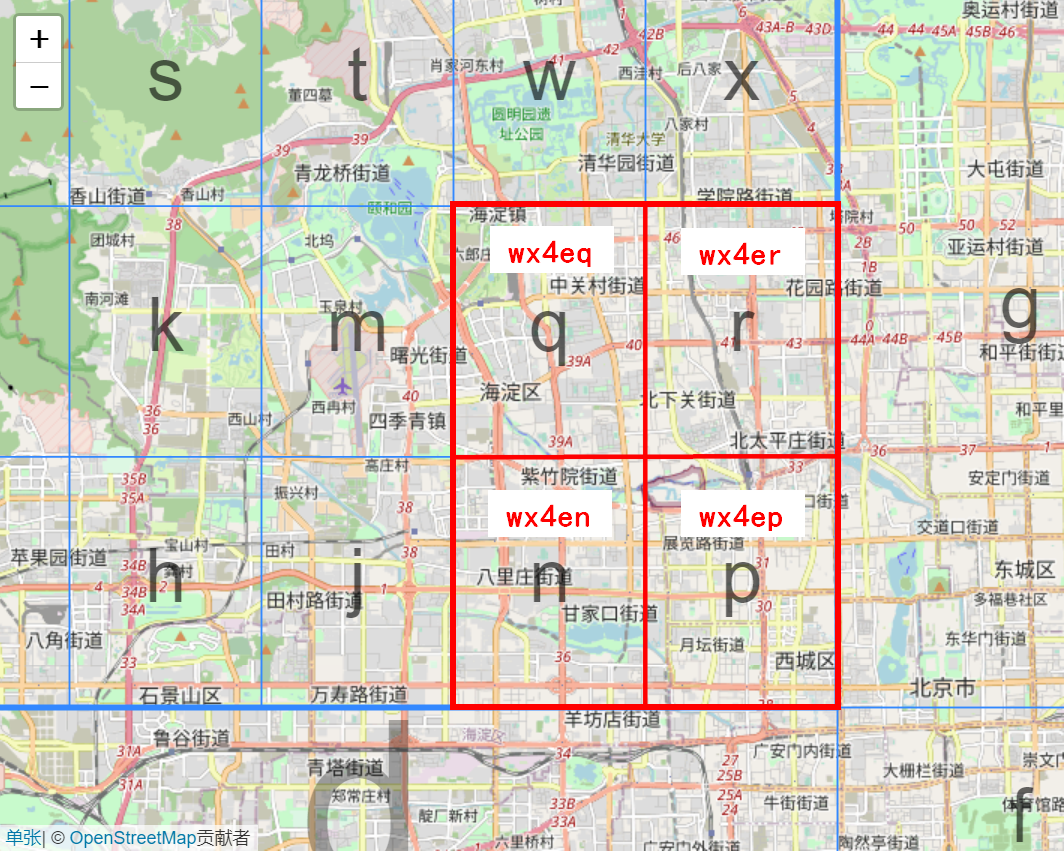
\includegraphics[width=0.6\textwidth]{undergraduate-thesis/images/FourRegions.png}
    \caption{以wx4e为前缀的四个五位编码区块示意图}
    \label{mapDataRegion-big}
\end{figure}

这四个区块对应的经纬度如表\ref{mapDataRegion-number}所示:

% 设置三线表
\begin{table}[ht]
    \linespread{1.5}
    \zihao{5}
    \centering
    \caption{区域经纬度范围}
    \label{mapDataRegion-number}
    \begin{tabular}{ccc}
    \toprule
    % \Xhline{1.5pt}
    区块的Geohash编码 & 经度范围 & 纬度范围 \\
    \midrule
    % \Xhline{0.5pt}  
    wx4eq & [116.279,116.323] & [39.947,39.991]\\
    wx4er & [116.323,116.367] & [39.947,39.991]\\
    wx4en & [116.279,116.323] & [39.903,39.947]\\
    wx4ep & [116.323,116.367] & [39.903,39.947]\\
    \bottomrule
    %\Xhline{1.5pt}
    \end{tabular}
\end{table}
% 结束设置三线表

\subsection{地图数据处理}

本文在处理地图数据时,主要采用地理信息处理软件ArcGIS和地理空间数据库PostgreSQL,具体涉及到的软件、插件及对应版本如表\ref{mapDataApp}所示:
\begin{table}[ht]
    \linespread{1.5}
    \zihao{5}
    \centering
    \caption{处理真实地图数据需要的软件、插件列表}
    \label{mapDataApp}
    \begin{tabular}{cc}
    \toprule
    % \Xhline{1.5pt}
    软件、插件名称 & 版本 \\
    \midrule
    % \Xhline{0.5pt}  
    ArcGIS & 10.8\\
    ArcGIS Editor for OSM & 10.8\\
    PostgreSQL & 6.21\\
    PostGIS & 3.3.2\\
    pgRouting & 3.4.2\\
    \bottomrule
    %\Xhline{1.5pt}
    \end{tabular}
\end{table}

使用以上工具处理地图数据时,需要经历以下步骤:用ArcGIS处理数据、用PostgreSQL处理数据、用脚本编码数据、向区块链上传数据。

1.用ArcGIS处理数据:

(a)数据裁剪:删去其他省市数据,缩减地图范围集中在北京区域,方便后续处理。

(b)要素转线:以两条道路的交叉点为基础打断道路,实现道路的分段效果。

(c)获取每个路段两端的经纬度:提前在ArcGIS中获取路段两端的经纬度数据,以便在PostgreSQL中直接筛选。

2.用PostgreSQL处理数据:

(a)导入数据库:将经由ArcGIS处理过的shp格式文件,以WGS84坐标系(SRID=4326)的投影方式导入数据库中。

(b)计算道路距离:在PostgreSQL中计算道路成本,并根据道路成本和道路经纬度建立路网拓扑回路。

(c)导出数据:在完成以上步骤中,PostgreSQL中应有如表\ref{mapData_Addproperty}中所示的新增项。然后在路网表中用SQL语句将所有筛选出的数据转为单行的Json语句,导出为一个Json文件。

3.用脚本编码数据:用JavaScript脚本处理导出的Json文件,主要是对每个路段的经纬度进行Geohash编码,形成一个包含Geohash编码信息的Json文件。

4.向区块链上传数据:将含有Geohash编码信息的Json文件上传给支持区域划分的树状区块链。该数据文件所在的Github仓库地址见附录D。

\begin{table}[ht]
    \linespread{1.5}
    \zihao{5}
    \centering
    \caption{从数据库中导出地图数据时必要的字段}
    \label{mapData_Addproperty}
    \begin{tabular}{cccc}
    \toprule
    % \Xhline{1.5pt}
    字段名称 & 注释 & 类型 & 示例\\
    \midrule
    % \Xhline{0.5pt}  
    start\_x & 该路段起始点经度 & numeric & 116.331388100 \\
    start\_y & 该路段起始点纬度 & numeric & 39.7695126000 \\
    end\_x & 该路段终止点经度 & numeric & 116.332542000 \\
    end\_y & 该路段终止点纬度 & numeric & 39.7695167000 \\
    cost & 道路的正向成本(代价) & double precision & 659.8882769759143 \\
    reverse\_cost & 道路的逆向成本(代价) & double precision & 659.8882769759143 \\
    source & 保存路径起始顶点的id(上一段道路) & integer & 830 \\
    target & 保存路径终止顶点的id(下一段道路) & integer & 835 \\
    \bottomrule
    %\Xhline{1.5pt}
    \end{tabular}
\end{table}

本章中使用的SQL查询语句见附录B。通过该语句导出的地图,包含了表\ref{mapData_pathpro}类型的道路数据:

\begin{table}[ht]
    \linespread{1.5}
    \zihao{5}
    \centering
    \caption{本文筛选的道路类型}
    \label{mapData_pathpro}
    \begin{tabular}{cccc}
    \toprule
    % \Xhline{1.5pt}
    道路等级 & \makecell{数据库中\\fclass字段值} & \makecell{数据库中\\code字段值} & 描述 \\
    \midrule
    % \Xhline{0.5pt}  
    国道、城市快速路 & trunk & 5112 & \makecell{城市道路系统中的快速路,\\重要性次于高速公路的公路。}\\
    省道、主干道 & primary & 5113 & \makecell{连接主要区域、城镇的道路,\\城市内较重要的市政道路。 }\\
    县道、次干道 & secondary & 5114 & \makecell{连接主要区域、村镇但不及省道的道路,\\城市道路系统中的次干道。} \\
    乡道、支路 & tertiary & 5115 & \makecell{连接村与村的道路,\\市政道路中狭窄的双向、单向2车道。}\\
    国道匝道 & trunk\_link & 5132 & 连接国道/快速路、更低级道路的连接路。\\
    省道匝道 & primary\_link & 5133 & 连接省道/主干道、更低级道路的连接路。\\
    县道匝道 & secondary\_link & 5134 & 连接县道/次干道、更低级道路的连接路。\\
    乡道匝道 & tertiary\_link & 5135 & 连接乡道/支路、更低级道路的连接路。\\
    \bottomrule
    %\Xhline{1.5pt}
    \end{tabular}
\end{table}

\section{本章小结}

本章聚焦于研究工作的数据部分,首先介绍了周畅的支持区域划分的树状区块链的设计方式,其次介绍了对实验室前人工作的复现过程,最后介绍了地图数据的获取和处理流程,为后续在实验室已有工作的基础上开展基于实时路况的A*算法的设计与测试打下了良好的基础。